\section*{Matched Vehicle Detection}
The local FP32 diagnostic applies each synthetic degradation at source size,
then compares direct detection, resize-only and restored views at 128 and 256,
and native restoration (Fig.~\ref{fig:resolution}). All branches return to
source geometry before the same $640\times640$ detector preprocessing.
Across eight labelled added-weather variants, the 256 restorer adds no new
matches and loses one relative to resize-only (19 versus 20 matches).
Native restoration recovers the rainy truck and misses the smoky truck.

The vehicle gallery below and the people comparison in
Fig.~\ref{fig:matched-128-people} show the 128-pixel controls: two labelled
scenes, five annotated objects and four weather variants.
Each row shares exactly the same degraded source pixels. The middle column
isolates resampling; the right adds the frozen Restormer. These examples show
recoveries, remaining misses and removed unmatched predictions. A third,
unlabelled camera scene contributes prediction counts only; the full
controls and timing scopes appear in Appendix~\ref{app:hardware}.

\medskip
\noindent\begin{minipage}{\linewidth}
\centering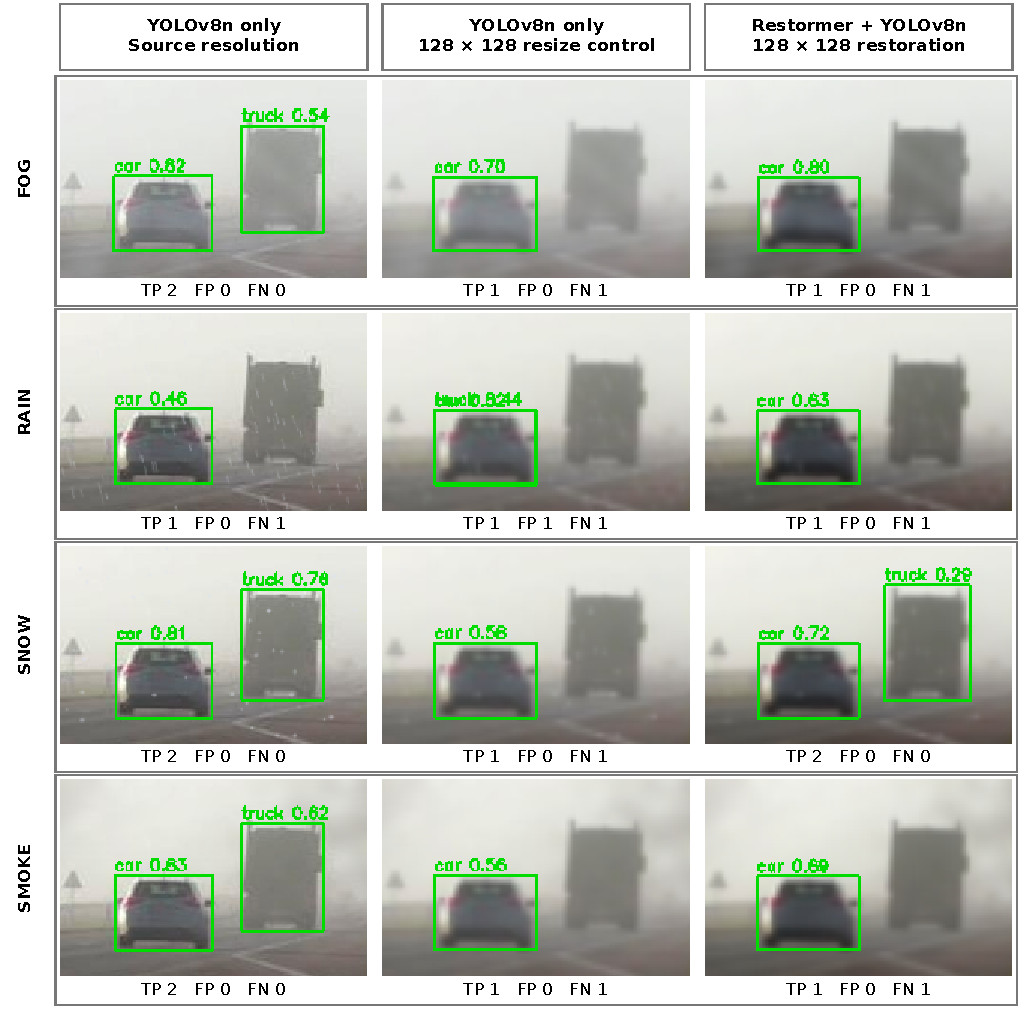
\includegraphics[width=\linewidth]{figures/matched_128_vehicles.pdf}
\captionof{figure}{Matched vehicle comparison: source-size YOLOv8n, a $128\times128$ resize-only canvas with YOLOv8n, and Restormer on the same $128\times128$ canvas followed by YOLOv8n. A common display crop retains both annotated vehicles and every saved prediction. TP/FP/FN use confidence 0.25 and class-aware IoU 0.50. Restoration recovers the truck relative to resize-only in snow, but it remains missed in fog, rain and smoke; the extra rain prediction in the resize control disappears. These saved CPU FP32 diagnostic overlays are not Nano benchmark frames.}
\label{fig:matched-128-vehicles}
\end{minipage}

\clearpage
